\documentclass[10pt,a4paper,twocolumn]{article}
\usepackage[utf8]{inputenc}
\usepackage[T1]{fontenc}
\usepackage[spanish,es-tabla]{babel}
\usepackage{geometry}
\geometry{margin=1.8cm,columnsep=0.7cm}
\usepackage{booktabs}
\usepackage{array}
\usepackage{url}
\usepackage{graphicx}
\usepackage{listings}
\lstset{basicstyle=\ttfamily\footnotesize, breaklines=true, columns=fullflexible}
\setlength{\parindent}{0pt}
\setlength{\parskip}{0.45em}
\setlength{\emergencystretch}{2em}

\begin{document}
\twocolumn[
\begin{minipage}{\textwidth}
\centering
{\LARGE\bfseries Caracterización y reducción de imágenes CCD\par}
\vspace{0.35em}
{\normalsize Daniel Soto Villada y Joan Mauricio Yanza Ruiz\par}
{\small [Afiliación institucional]\par}
{\normalsize [Fecha]\par}
\vspace{0.7em}
\textbf{Resumen}\par
\small
% Pendiente de completar.
\end{minipage}
\vspace{1em}
]

\section{Introducción}
% Pendiente de desarrollar.

\section{Materiales y métodos}
\subsection{Bitácora de observación}
La información de las Tablas~\ref{tab:bitacora} y~\ref{tab:noches} se extrajo
directamente de las cabeceras FITS con las tareas \texttt{imhead} y
\texttt{hselect} de IRAF:

\begin{lstlisting}
ecl> imhead Bias/domeflat_Bias_1_secs_001.fits l+
ecl> imhead MEL25_Light_B_90_secs_001.fits l+
ecl> hselect Bias/*.fits,Dark/*.fits,domeflat_B/*.fits,domeflat_V/*.fits,MEL25*.fits "$I,IMAGETYP,FILTER,EXPTIME,DATE-OBS,UT,CCD-TEMP,INSTRUME" yes > bitacora.txt
ecl> !cat bitacora.txt
\end{lstlisting}

\noindent\textbf{Parámetros fijos leídos de las cabeceras:} observatorio La
Silla; cámara CCD-FLI ML0900 (alias TUCAN, \texttt{INSTRUME='FLI CCD'});
adquisición generada por INDI; binning $1\times1$; píxel de 12\,$\mu$m; escala
de 8.252''/píxel; formato de $3056\times3056$ píxeles con dos regiones de
overscan (sobre filas y sobre columnas).

\begin{table*}[t]
\centering
\caption{Bitácora de observación resumida por tipo de imagen. Las horas están
en UT y corresponden al inicio y al cierre de cada serie.}
\label{tab:bitacora}
\footnotesize
\setlength{\tabcolsep}{3pt}
\begin{tabular}{@{}>{\raggedright\arraybackslash}p{4.3cm}lcccllc@{}}
\toprule
Archivo (patrón de nombres) & Tipo (\texttt{IMAGETYP}) & $N$ & $t_{\mathrm{exp}}$\,(s) & Filtro & Fecha y hora (UT) & $T_{\mathrm{CCD}}$\,($^\circ$C) \\
\midrule
\path{Bias/domeflat_Bias_1_secs_001-047.fits} & zero (bias) & 47 & 0  & Ha, X, V, I, U & 2024-10-25/26, 21:46:54--02:53:39 & $-24.94$ \\
\path{Dark/MEL25_Dark_90_secs_001-005.fits}   & dark        & 5  & 90 & I              & 2024-12-04, 04:28:54--04:35:41     & $-25.00$ \\
\path{domeflat_B/domeflat_Flat_B_90_secs_001-005.fits} & flat & 5 & 90 & B              & 2024-10-25, 21:53:02--21:59:53     & $-24.94$ \\
\path{domeflat_V/domeflat_Flat_V_40_secs_001-005.fits} & flat & 5 & 40 & V              & 2024-10-25, 22:01:37--22:05:08     & $-24.94$ \\
\path{MEL25_Light_B_90_secs_001.fits}         & object      & 1  & 90 & B              & 2024-12-04, 04:04:09               & $-25.00$ \\
\path{MEL25_Light_V_90_secs_001.fits}         & object      & 1  & 90 & V              & 2024-12-04, 04:04:09               & $-25.00$ \\
\bottomrule
\end{tabular}
\end{table*}

\begin{table*}[t]
\centering
\caption{Reconstrucción cronológica de las noches de observación (Paso 1).}
\label{tab:noches}
\footnotesize
\begin{tabular}{@{}lllccc@{}}
\toprule
Noche (UT) & Hora (UT) & Tipo de imagen & Filtro & $N$ & $t_{\mathrm{exp}}$\,(s) \\
\midrule
2024-10-25 & 21:46:54--21:50:54 & bias          & Ha & 20 & 0  \\
           & 21:52:34--21:52:47 & bias          & X  & 2  & 0  \\
           & 21:53:02--21:59:53 & dome flat     & B  & 5  & 90 \\
           & 22:01:37--22:05:08 & dome flat     & V  & 5  & 40 \\
           & 22:05:59--22:06:12 & bias          & V  & 2  & 0  \\
           & 23:01:52--23:02:05 & bias          & I  & 2  & 0  \\
2024-10-26 & 02:49:28--02:53:39 & bias          & U  & 21 & 0  \\
\midrule
2024-12-04 & 04:04:09           & ciencia MEL25 & B  & 1  & 90 \\
           & 04:04:09           & ciencia MEL25 & V  & 1  & 90 \\
           & 04:28:54--04:35:41 & dark          & I  & 5  & 90 \\
\bottomrule
\end{tabular}
\end{table*}

\noindent\textbf{Notas de la bitácora:}
\begin{itemize}\footnotesize
\item El archivo \path{Bias/Zero.fits} duplica el marco 001 (mismo \texttt{DATE-OBS}); se contabilizó una sola vez (47 bias únicos).
\item El filtro anotado en los bias (Ha, X, V, I, U) corresponde a la posición de la rueda de filtros al momento de leer el cero; el nivel de bias no depende del filtro.
\item Los darks se tomaron con la rueda en I; la corriente oscura es independiente del filtro.
\item Ambas imágenes de ciencia reportan el mismo \texttt{UT} en sus cabeceras (para B, \texttt{UTMIDDLE} = 2024-12-04T04:04:54.82).
\end{itemize}

\subsection{Ganancia y ruido de lectura}
La ganancia $g$ y el ruido de lectura RN se determinaron por filtro mediante el
método de la varianza de diferencias: con un par de dome flats y un par de bias
se construyen imágenes de diferencia, que eliminan toda estructura espacial
(iluminación, polvo, viñeteo) y conservan únicamente el ruido:

\begin{equation}
\sigma^2_F = \frac{\mathrm{Var}(F_1-F_2)}{2}, \qquad
\sigma^2_B = \frac{\mathrm{Var}(B_1-B_2)}{2},
\end{equation}
\begin{equation}
g = \frac{\bar{F}-\bar{B}}{\sigma^2_F-\sigma^2_B}, \qquad
\mathrm{RN} = g\,\sigma_B .
\end{equation}

\noindent Las estadísticas se calcularon sobre la región central
$[1000:2000]\times[1000:2000]$ para excluir overscan y bordes. Para el filtro B
se usaron los flats 001--002 con los bias 019--020 (contiguos en el tiempo);
para el filtro V, los flats 001--002 con los bias 023--024. El cálculo se
realizó con un script en Python (\texttt{astropy}/\texttt{numpy}).

\subsection{Ajuste y sustracción del overscan bidimensional}
Las imágenes del detector CCD-FLI ML0900 (TUCAN) presentan dos regiones de
overscan: una franja vertical en las columnas izquierdas y una franja
horizontal en las filas inferiores. Estas regiones no corresponden al área
fotosensible del detector, sino a píxeles ficticios que permiten monitorear
el nivel electrónico de lectura. Para corregir este efecto se emplearon las
tareas \texttt{colbias} y \texttt{linebias} del paquete \texttt{bias} de
IRAF, que ajustan un polinomio de Chebyshev al nivel de lectura en cada
franja y lo sustraen de la imagen científica.

\subsubsection{Identificación de las regiones de overscan}

Para determinar los límites exactos de las regiones de overscan se analizó
el perfil medio de columnas y filas de una imagen dome flat en filtro B
(\texttt{domeflat\_B/domeflat\_Flat\_B\_90\_secs\_001.fits}) mediante un
script en Python con \texttt{astropy}:

\begin{lstlisting}[language=Python]
import numpy as np
from astropy.io import fits

img = 'domeflat_B/domeflat_Flat_B_90_secs_001.fits'
d = fits.getdata(img).astype(float)
nc, nr = d.shape[1], d.shape[0]

col = d.mean(axis=0)    # perfil a lo largo de columnas
row = d.mean(axis=1)    # perfil a lo largo de filas
nivel_col = np.median(col[nc//3:2*nc//3])
nivel_row = np.median(row[nr//3:2*nr//3])

def limites(perfil, nivel):
    dentro = np.where(perfil > nivel*0.5)[0]
    return dentro[0]+1, dentro[-1]+1

c1, c2 = limites(col, nivel_col)
r1, r2 = limites(row, nivel_row)

print(f'Area cientifica columnas: {c1}:{c2}')
print(f'Area cientifica filas:    {r1}:{r2}')
\end{lstlisting}

\noindent La salida del script indicó:

\begin{itemize}
\item \textbf{Overscan de columnas (primera región):} franja vertical
izquierda, columnas 1:35, con nivel de lectura $\approx 1020$ ADU.
\item \textbf{Overscan de filas (segunda región):} franja horizontal
inferior, filas 1:20, con nivel de lectura $\approx 1208$ ADU.
\item \textbf{Área científica bruta:} columnas 36:3056, filas 21:3056.
\end{itemize}

\subsubsection{Corrección de la primera región (columnas) con \texttt{colbias}}

La tarea \texttt{colbias} ajusta un polinomio de Chebyshev al nivel de
lectura en la franja de overscan de columnas, lo sustrae de cada fila y
recorta la imagen al área científica definida por \texttt{trimsection}.
Los parámetros utilizados fueron:

\begin{lstlisting}
noao
imred
bias
unlearn colbias
colbias domeflat_B/domeflat_Flat_B_90_secs_001.fits TrmFlatB001.fits \
  bias="[1:35,21:3056]" trim="[36:3056,1:3056]" \
  function=chebyshev order=1 interactive=no median=no \
  low_rej=3. high_re=3.
\end{lstlisting}

\noindent\textbf{Descripción de parámetros:}
\begin{itemize}
\item \texttt{bias="[1:35,21:3056]"}: región de overscan de columnas
utilizada para estimar el nivel de lectura. Se excluyen las filas 1:20
para evitar contaminación con el overscan de filas.
\item \texttt{trim="[36:3056,1:3056]"}: área científica que se conserva
(todas las filas, ya que el overscan de filas se corrige después).
\item \texttt{function=chebyshev, order=1}: ajuste polinomial de primer
orden al nivel de lectura a lo largo de las filas.
\item \texttt{interactive=no, median=no}: se desactiva el ajuste
interactivo y el uso de mediana.
\item \texttt{low\_rej=3., high\_rej=3.}: rechazo de píxeles a más de
3$\sigma$ del ajuste.
\end{itemize}

\noindent La figura~\ref{fig:antes_colbias} muestra el perfil horizontal
de la imagen original (antes de \texttt{colbias}), donde se observa el
salto en las columnas 1:35. La figura~\ref{fig:despues_colbias} muestra el
perfil de la imagen recortada (después de \texttt{colbias}), donde la
franja de overscan de columnas ha sido eliminada.

\begin{figure}[ht]
\centering
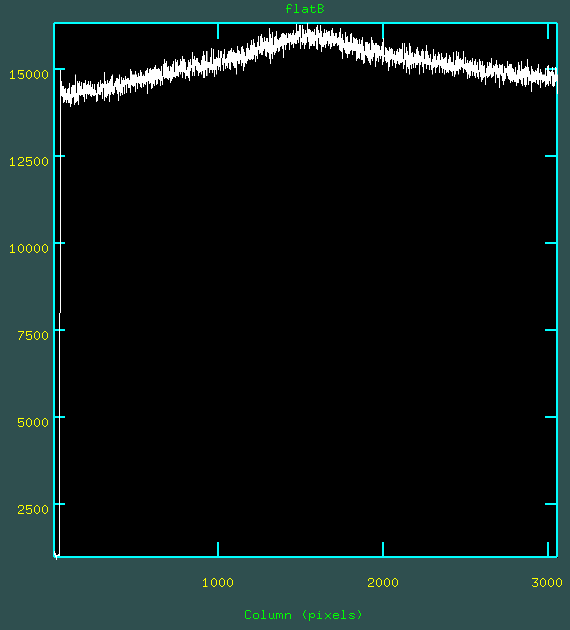
\includegraphics[width=\linewidth,height=0.28\textheight,keepaspectratio]{imagenes/perfil_antes_colbias.png}
\caption{Perfil horizontal de \texttt{domeflat\_Flat\_B\_90\_secs\_001.fits}
antes de aplicar \texttt{colbias}. Se observa el salto en las columnas
1:35 correspondiente al overscan de columnas (nivel $\approx 1020$ ADU).}
\label{fig:antes_colbias}
\end{figure}

\begin{figure}[ht]
\centering
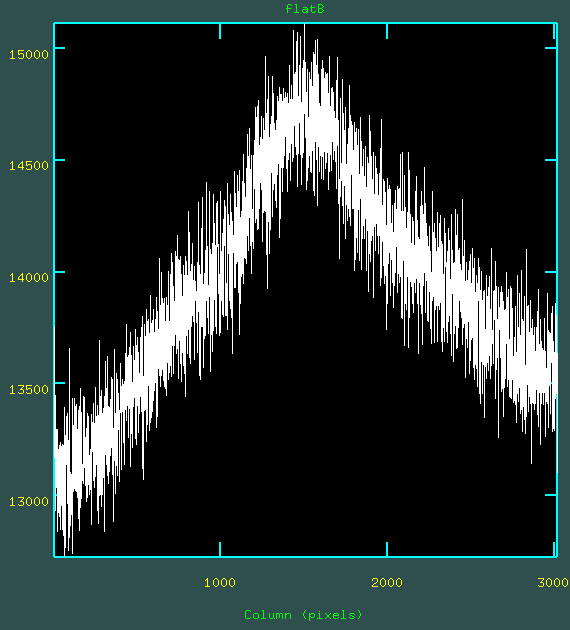
\includegraphics[width=\linewidth,height=0.28\textheight,keepaspectratio]{imagenes/perfil_despues_colbias.png}
\caption{Perfil horizontal de \texttt{TrmFlatB001.fits} después de aplicar
\texttt{colbias}. La franja de overscan de columnas ha sido sustraída y
recortada. La forma de domo observada corresponde al gradiente de
iluminación del dome flat.}
\label{fig:despues_colbias}
\end{figure}

\subsubsection{Corrección de la segunda región (filas) con \texttt{linebias}}

Sobre la imagen ya recortada en columnas (\texttt{TrmFlatB001.fits}, de
3021 columnas $\times$ 3056 filas), se aplicó \texttt{linebias} para
corregir el overscan de filas:

\begin{lstlisting}
unlearn linebias
linebias TrmFlatB001.fits Trm2FlatB001.fits \
  bias="[1:3021,1:20]" trim="[1:3021,21:3056]" \
  function=chebyshev order=1 interactive=no median=no \
  low_rej=3. high_re=3.
\end{lstlisting}

\noindent La figura~\ref{fig:antes_linebias} muestra el perfil vertical
de \texttt{TrmFlatB001.fits} (antes de \texttt{linebias}), donde se
observa el salto en las filas 1:20. La figura~\ref{fig:despues_linebias}
muestra el perfil de la imagen final (\texttt{Trm2FlatB001.fits}), donde
ambas regiones de overscan han sido eliminadas.

\begin{figure}[ht]
\centering
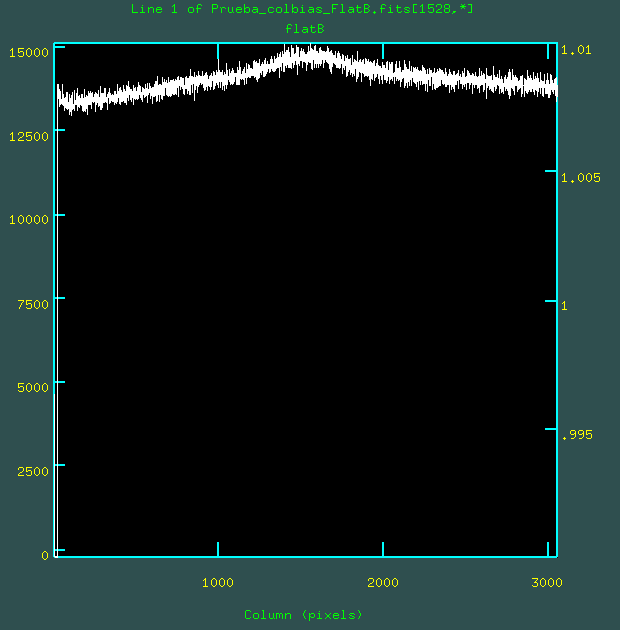
\includegraphics[width=\linewidth,height=0.28\textheight,keepaspectratio]{imagenes/perfil_antes_linebias.png}
\caption{Perfil vertical de \texttt{TrmFlatB001.fits} antes de aplicar
\texttt{linebias}. Se observa el salto en las filas 1:20 correspondiente
al overscan de filas (nivel $\approx 1208$ ADU).}
\label{fig:antes_linebias}
\end{figure}

\begin{figure}[ht]
\centering
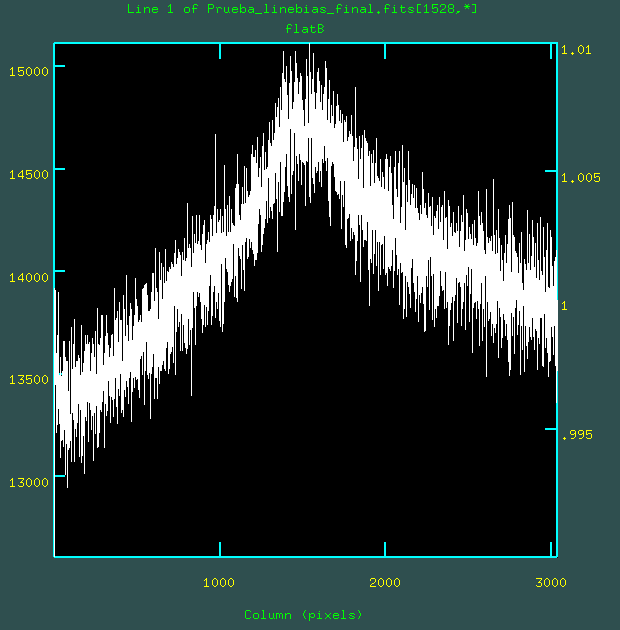
\includegraphics[width=\linewidth,height=0.28\textheight,keepaspectratio]{imagenes/perfil_despues_linebias.png}
\caption{Perfil vertical de \texttt{Trm2FlatB001.fits} después de aplicar
\texttt{linebias}. Ambas regiones de overscan han sido sustraídas y
recortadas. La imagen final tiene dimensiones 3021 $\times$ 3036 píxeles.}
\label{fig:despues_linebias}
\end{figure}

\subsubsection{Aplicación por lotes a todas las imágenes}

Una vez verificados los parámetros con la imagen de prueba, se procesaron
las 65 imágenes (47 bias, 5 darks, 5 flats B, 5 flats V y 2 ciencias)
mediante un script \texttt{overscan\_lote.cl}:

\begin{lstlisting}
# overscan_lote.cl
noao
imred
bias

!ls Bias/Zero.fits Bias/domeflat_Bias_1_secs_*.fits Dark/*.fits \
  domeflat_B/*.fits domeflat_V/*.fits MEL25*.fits > input
!sed 's|.*/||; s|^|Trm|' input > output

colbias @input @output bias="[1:35,21:3056]" trim="[36:3056,1:3056]" \
  function=chebyshev order=1 interactive=no median=no \
  low_rej=3. high_re=3.

!ls Trm*.fits > input2
!sed 's|^|Lb|' input2 > output2

linebias @input2 @output2 bias="[1:3021,1:20]" trim="[1:3021,21:3056]" \
  function=chebyshev order=1 interactive=no median=no \
  low_rej=3. high_re=3.

!ls Lb*.fits
\end{lstlisting}

\section{Resultados}
\subsection{Ganancia y ruido de lectura}
\begin{table}[ht]
\centering
\caption{Resultados del método de la varianza de diferencias por filtro.}
\label{tab:ganancia}
\begin{tabular}{lcc}
\toprule
Cantidad & Filtro B & Filtro V \\
\midrule
$\bar{F}$ (ADU)              & 15464.78 & 15223.71 \\
$\bar{B}$ (ADU)              & 1005.50  & 1006.33  \\
$S=\bar{F}-\bar{B}$ (ADU)    & 14459.28 & 14217.37 \\
$\sigma^2_F$ (ADU$^2$)       & 10049.80 & 9835.71  \\
$\sigma^2_B$ (ADU$^2$)       & 44.10    & 45.18    \\
\midrule
$g$ (e$^-$/ADU)              & 1.445    & 1.452    \\
RN (e$^-$)                   & 9.60     & 9.76     \\
\bottomrule
\end{tabular}
\end{table}

\noindent\textbf{Valor adoptado:} $g = 1.45 \pm 0.01$~e$^-$/ADU y
RN $= 9.7 \pm 0.1$~e$^-$. El acuerdo entre filtros (menor al 2\,\%) es
esperable, pues ambos parámetros son propiedades del detector y su
electrónica, no del filtro; esto valida el método. Como verificación, la
varianza de disparo esperada $S/g \approx 10006$~ADU$^2$ reproduce la
varianza del flat una vez restado el aporte de lectura ($\sigma^2_F -
\sigma^2_B$).

\subsection{Verificación de la corrección del overscan}
\noindent La verificación final confirmó que todas las imágenes
\texttt{LbTrm*.fits} tienen dimensiones [3021,3036] y carecen de las
franjas de overscan visibles en las imágenes originales.

\section{Discusión}
% Pendiente de desarrollar.

\section{Conclusiones}
% Pendiente de desarrollar.

\section*{Referencias}
% Agregar aquí las referencias utilizadas.

\end{document}